%
% friedmann-materie.tex -- Funktion S_\kappa(r) 
%
% (c) 2017 Prof Dr Andreas Müller, Hochschule Rapperswil
%
\documentclass[tikz]{standalone}
\usepackage{times}
\usepackage{txfonts}
\usepackage{pgfplots}
\usetikzlibrary{arrows,intersections}
\begin{document}
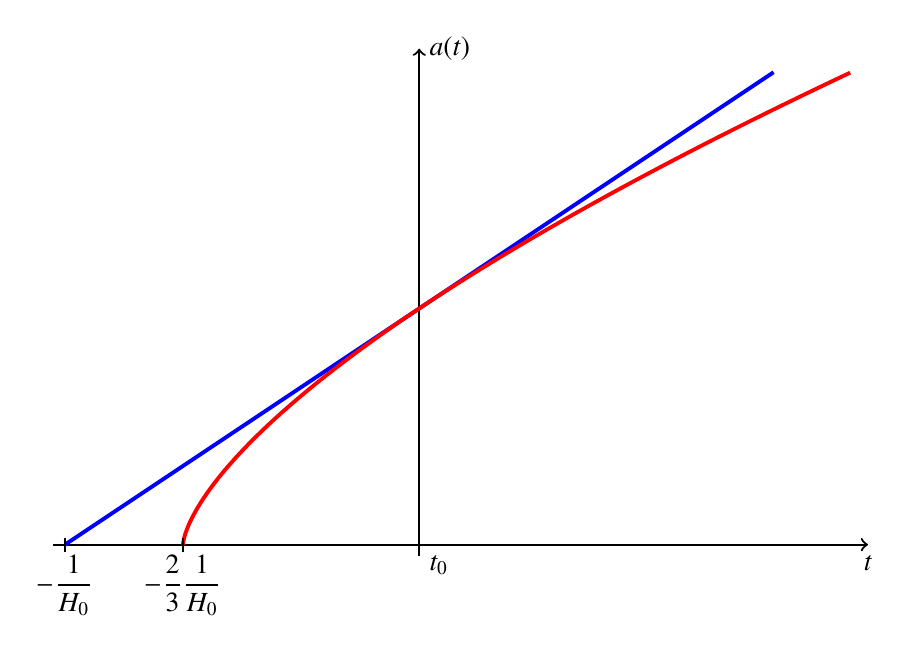
\begin{tikzpicture}[thick,scale=3]
\coordinate (O) at (0,0);

\draw[->] (-0.55, 0   )--(2.9,  0  ) coordinate[label = {below:$t$}];
\draw[->] ( 1,   -0.05)--(1  ,  2.1) coordinate[label = {right:$a(t)$}];

\draw[blue,line width=1.4] (-0.5,0)--(2.5,2);
\draw[red,domain=0:2.00,samples=200,line width=1.4] plot ({\x*sqrt(\x)},\x);

\node at ( 1,0) [below right] {$t_0$};
\node at (-0.5,0) [below] {$\displaystyle-\frac1{H_0}$};
\node at ( 0,0) [below] {$\displaystyle-\frac23\frac1{H_0}$};

\draw (0,-0.03)--(0,0.03);
\draw (-0.5,-0.03)--(-0.5,0.03);

\end{tikzpicture}
\end{document}


